%\documentclass{cmspaper}
%\begin{document}
%
\section{Cut Optimization} \label{sec:cutOptimization}

Eight criteria are used to select events, as described in section XXX.  These are the $p_T$ of the two leading jets and two leading electrons, the $\eta$ of the electrons and $\eta$ of the jets, the invariant mass of the two leading electrons and the $S_T$, the sum of the $p_T$ of the two leading electrons and jets.  

The optimal cut values for the selection criteria are chosen in order to maximize the significance of the signal, calculated as (number of signal events) / (number of signal plus background events).
A range of cut values to be tested for each variable is chosen and the number of events passing the selection is calculated for each combination of possible values for each variable.  The combination with the 
highest significance value is taken as the optimized values.

The Bayesian method to estimate the upper limit on the cross section of the signal is a more appropriate measure of the quality of a cut value in analysis such as this, as is described in section XXX.  
This calculation, however, is much more time consuming and is not a feasible method of optimization for all 8 variables.  A hard cut on the $S_T$ of the event shows the strongest discriminating power of the selection criteria.  
Therefore this variable alone was optimized to minimize the estimate of the upper limit on the signal cross section based on the Bayesian approach described in section XX.  

Figure \ref{fig:optimization} shows the variation on the upper limit of the cross section as a function of varying $S_T$ cut on a 400 GeV leptoquark sample with standard model background estimates for $100 pb_{-1}$.  The optimization was done first using only the statistical uncertainties from the number of signal and background events, and then adding an estimate of 10\% and 20\% to the uncertainty in the number of events due to systematic effects.  The cross section limit changes, naturally, but the optimized cut on $S_T$ does not change.  

The results for the optimal cut values for the electron and jet $p_T$ are consistently the lowest value in the scanned range.  However, an increase in the cut value of the object $p_T$ is seen to have only a small effect on the significance of the signal.  Higher than optimal cut values for the $p_T$ of the jets are chosen in order to reduce the effect of initial and final state radiation and the effects of calorimeter noise.  The electron $p_T$ cut values are chosen to agree with those used in the HEEP analysis.

Table XXX in section XXX shows the values chosen for each of the selection criteria.  

\begin{figure}[htbp]
  \begin{center}
      \resizebox{11cm}{!}{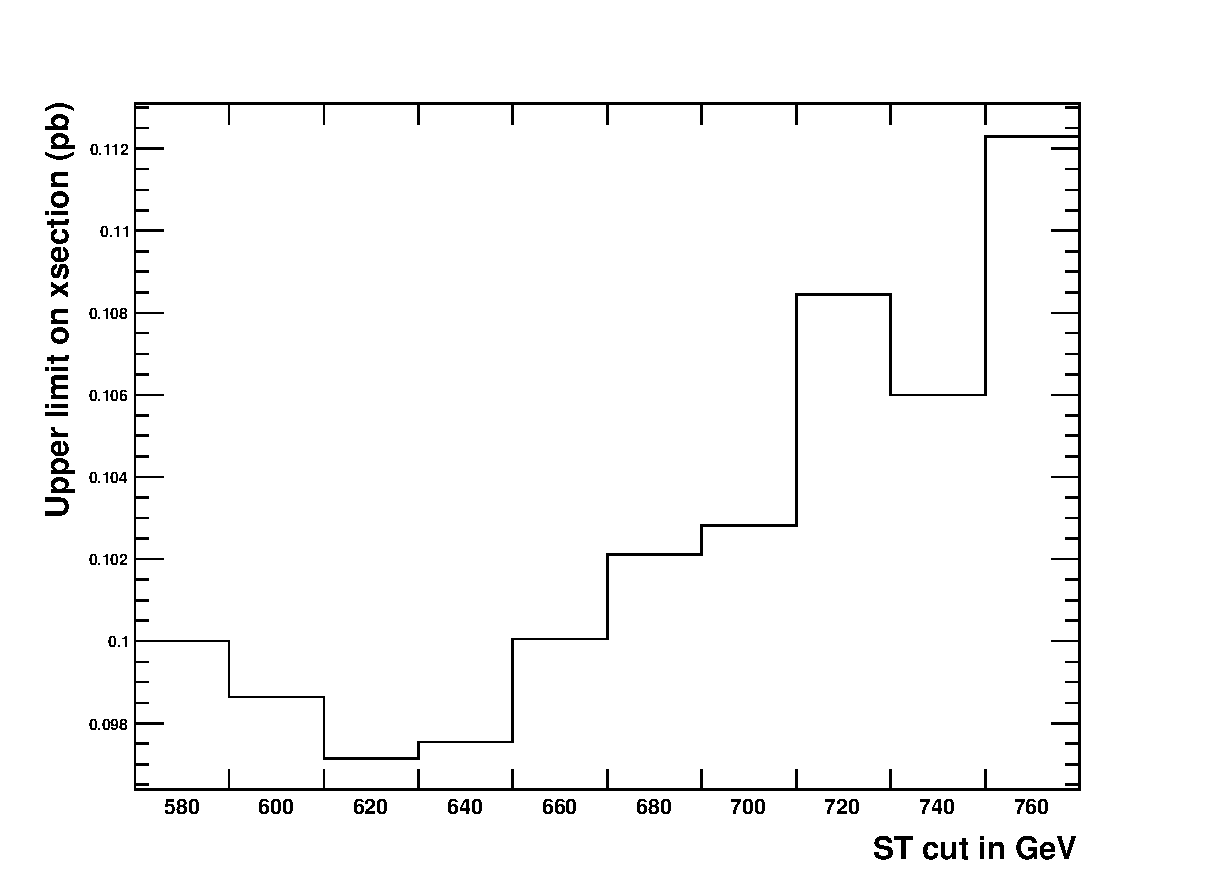
\includegraphics{plots/xSecLimit_M400.eps}} \\
    \caption{\small \sl Upper limit on the signal cross section for a range of $S_T$ cuts }
    \label{fig:optimization}
  \end{center}
\end{figure}

%\end{document}
